% ============================================================
% Corrigé enseignant : TD Équations différentielles du premier ordre (v2.0)
% Pôle Formation UIMM - CVDL - BTS Industriel - S. JAUBERT
% Énoncé : MOD06_EDL1_TD_v2_0 (compiler l'énoncé AVANT le corrigé :
% les numéros de page de l'énoncé sont lus dans son fichier .aux).
% ============================================================
\documentclass[a4paper,11pt]{article}
\usepackage[utf8]{inputenc}
\usepackage[T1]{fontenc}
\IfFileExists{french.ldf}{\usepackage[french]{babel}}{}
\usepackage{helvet}
\renewcommand{\familydefault}{\sfdefault}
\renewcommand{\ttdefault}{lmtt}
\usepackage[top=2cm, bottom=3cm, left=2cm, right=2cm, headheight=14pt, footskip=1.6cm]{geometry}
\usepackage{amsmath,amssymb}
\usepackage{graphicx}
\usepackage[dvipsnames,table]{xcolor}
\usepackage{tikz}
\usetikzlibrary{arrows.meta}
\usepackage{pgfplots}
\pgfplotsset{compat=1.18}
\usepackage[most]{tcolorbox}
\usepackage{fancyhdr}
\usepackage{enumitem}
\usepackage{array,tabularx,needspace}
\usepackage{lastpage}
\usepackage{xr}
\externaldocument[E-]{MOD06_EDL1_TD_v2_0}
\usepackage{hyperref}

\definecolor{uimmblue}{HTML}{005C85}
\definecolor{uimmred}{HTML}{D31326}
\definecolor{uimmlightblue}{HTML}{E8F1F8}
\definecolor{uimmgray}{HTML}{333333}
\definecolor{uimmlightgray}{HTML}{F5F5F5}
\definecolor{uimmgreen}{HTML}{2E7D32}
\hypersetup{colorlinks=true, linkcolor=uimmblue, urlcolor=uimmblue}
\setlength{\parindent}{0pt}
\setlength{\parskip}{3pt}

\setlist[enumerate,1]{label={\color{uimmblue}\textbf{\arabic*.}}, leftmargin=*, itemsep=3pt}
\setlist[enumerate,2]{label=\alph*), itemsep=2pt}
\setlist[itemize,1]{label={\color{uimmblue}\textbullet}}

\pagestyle{fancy}
\fancyhf{}
\renewcommand{\headrulewidth}{0pt}
\fancyfoot[C]{\small\renewcommand{\arraystretch}{1.3}%
\begin{tabularx}{\textwidth}{|>{\centering\arraybackslash\itshape}X|>{\centering\arraybackslash}p{1.8cm}|>{\centering\arraybackslash}p{3.6cm}|>{\centering\arraybackslash}p{1.9cm}|}
\hline
Corrigé enseignant -- MOD06 Équations différentielles -- [S01] & {\scriptsize\itshape Auteur :}\newline SJ & MAJ du 07/10/2026\newline{\color{uimmblue}Version 2.0} & Page :\newline \thepage/\pageref*{LastPage}\\
\hline
\end{tabularx}}

\newcommand{\partie}[1]{\needspace{16\baselineskip}\vspace{6pt}%
\begin{tcolorbox}[colback=uimmblue, colframe=uimmblue, sharp corners, boxrule=0pt, left=10pt, top=4pt, bottom=4pt]
{\color{white}\large\bfseries #1}
\end{tcolorbox}}
% \cor{n}{titre}
\newcommand{\cor}[2]{\needspace{8\baselineskip}\vspace{8pt}%
\begin{tcolorbox}[colback=uimmlightblue, colframe=uimmblue, boxrule=0.8pt, arc=2pt, left=6pt, right=6pt, top=3pt, bottom=3pt]
{\color{uimmblue}\bfseries Exercice #1 : #2}\hfill{\small\color{uimmred}\bfseries Énoncé p.~\pageref*{E-exo:#1}}
\end{tcolorbox}}
\newcommand{\vig}[1]{\par{\small\color{uimmred}\textbf{Vigilance.} #1}\par}
\newcommand{\res}[1]{\colorbox{uimmlightblue}{$\displaystyle #1$}}
\newcommand{\py}{{\color{uimmred}\small\bfseries[Python]}}
\newenvironment{sortie}{\par\begin{tcolorbox}[colback=uimmlightgray, colframe=uimmgray, boxrule=0.5pt, arc=1pt, left=6pt, top=2pt, bottom=2pt, fontupper=\ttfamily\small]}{\end{tcolorbox}}
\newcommand{\dd}{\mathrm{d}}

\begin{document}

% ============================================================
% EN-TÊTE PR3
% ============================================================
\noindent{\renewcommand{\arraystretch}{1.1}%
\begin{tabularx}{\textwidth}{|>{\centering\arraybackslash}m{2.9cm}|>{\centering\arraybackslash}m{4.3cm}|>{\centering\arraybackslash}X|}
\hline
\rule{0pt}{2.4cm}
\includegraphics[height=2.2cm]{logo_uimm_placeholder.jpg} &
{\bfseries\large CFAI CENTRE}\newline{\footnotesize 74, Route Nationale\newline La Chapelle St Mesmin\newline orleans@poleformation-\newline uimmcvdl.fr} &
{\Large\bfseries\color{uimmblue}Corrigé enseignant}\newline{}{\large\bfseries TD : Équations différentielles du premier ordre}\newline{}{\small Version 2.0 -- document réservé au formateur}\\
\hline
\end{tabularx}}

\vspace{6pt}
\begin{tcolorbox}[colback=uimmlightgray, colframe=uimmgray, boxrule=0.6pt, arc=2pt, left=8pt, right=8pt, top=4pt, bottom=4pt]
\small
\textbf{Mode d'emploi.} Chaque exercice renvoie à sa page dans l'énoncé (MOD06\_EDL1\_TD\_v2\_0). Les résultats à retenir sont surlignés en bleu. Les sorties des programmes \py{} ont été obtenues en exécutant les codes de l'énoncé avec Python 3. Les mentions \textcolor{uimmred}{\textbf{Vigilance}} signalent les erreurs fréquentes.

\smallskip
\textbf{Durée indicative.} Partie A : 1\,h 30. Partie B : 3\,h. Partie C : 4\,h à 5\,h (la partie C peut être répartie sur plusieurs séances, ou servir d'approfondissement pour les plus rapides).

\smallskip
\textbf{Correspondance avec la version 1.} Ex.~0.1 $\to$ ex.~6 ; ex.~0.2 $\to$ ex.~7 ; ex.~0.3 $\to$ ex.~8 ; ex.~0.4 $\to$ ex.~9 ; ex.~0.5 $\to$ ex.~14 (modèle de Torricelli) ; ex.~0.6 $\to$ ex.~15.
\end{tcolorbox}

% ============================================================
\partie{Partie A : échauffement}
% ============================================================

\cor{1}{Reconnaître une équation différentielle}
\begin{enumerate}
\item
\begin{center}\renewcommand{\arraystretch}{1.35}\small
\begin{tabular}{|l|c|c|c|c|}
\hline
\rowcolor{uimmlightblue}\textbf{Équation} & \textbf{Ordre} & \textbf{Linéaire} & \textbf{Coef. constants} & \textbf{Homogène}\\ \hline
(a) $3y' + 6y = 0$ & 1 & oui & oui & oui \\ \hline
(b) $y' = 0{,}2\,y + 4$ & 1 & oui & oui & non \\ \hline
(c) $y' + t\,y = 0$ & 1 & oui & non & oui \\ \hline
(d) $h' = -0{,}5\sqrt{h}$ & 1 & non & sans objet & sans objet \\ \hline
(e) $y'' + 4y = 0$ & 2 & oui & oui & oui \\ \hline
(f) $v' = 9{,}81 - 0{,}04\,v^2$ & 1 & non & sans objet & sans objet \\ \hline
(g) $L\,i' + R\,i = E$ & 1 & oui & oui & non ($E \neq 0$) \\ \hline
\end{tabular}
\end{center}
\item (a) $y' + 2y = 0$ : $\alpha = 2$. \quad (b) $y' - 0{,}2\,y = 4$ : $\alpha = -0{,}2$. \quad (g) $i' + \dfrac{R}{L}\,i = \dfrac{E}{L}$ : $\alpha = \dfrac{R}{L}$.
\end{enumerate}
\vig{En (b), le terme en $y$ est passé à gauche : $\alpha$ est négatif. En (c), l'équation est linéaire mais son coefficient dépend de $t$ : la formule $C\,e^{-\alpha t}$ ne s'applique pas.}

\cor{2}{Équations homogènes}
\begin{enumerate}
\item $\alpha = 3$, $y = C\,e^{-3t}$, $y(0) = C = 2$ : \res{y(t) = 2\,e^{-3t}}.
\item $y' - 0{,}5\,y = 0$, $\alpha = -0{,}5$ : $y = C\,e^{0{,}5t}$, $C = 5$ : \res{y(t) = 5\,e^{0{,}5t}} (fonction croissante).
\item $y' + 4y = 0$ : $y = C\,e^{-4t}$. $y(1) = C\,e^{-4} = 4$ donne $C = 4\,e^{4} \approx 218{,}4$ : \res{y(t) = 4\,e^{-4(t-1)}}.
\item $u' + 10\,u = 0$ : \res{u(t) = 12\,e^{-10t}} ; $u(0{,}2) = 12\,e^{-2} \approx \res{1{,}62\ \text{V}}$.
\end{enumerate}
\vig{Question 3 : beaucoup écrivent $C = 4$. La condition porte sur $t = 1$, il faut résoudre $C\,e^{-4} = 4$.}

\cor{3}{Second membre constant}
\begin{enumerate}
\item $y_p = 3$, $y = C\,e^{-2t} + 3$, $y(0) = 0 \Rightarrow C = -3$ : \res{y(t) = 3 - 3\,e^{-2t}} ; $y_\infty = 3$, $\tau = 0{,}5$.
\item $y' + 0{,}25\,y = 5$ : $y_p = 20$, $y = C\,e^{-t/4} + 20$, $C = 30$ : \res{y(t) = 20 + 30\,e^{-t/4}} ; $y_\infty = 20$, $\tau = 4$ (décroissance de $50$ vers $20$).
\item $y' + 0{,}1\,y = 3$ : $y_p = 30$, $C = 10 - 30 = -20$ : \res{y(t) = 30 - 20\,e^{-0{,}1t}} ; $y_\infty = 30$, $\tau = 10$.
\end{enumerate}

\cor{4}{Lire la réponse d'un capteur de température}
\begin{enumerate}
\item $T_0 = 20\,^\circ$C ; $T_\infty = 200\,^\circ$C.
\item $T_0 + 0{,}63\,(T_\infty - T_0) = 20 + 0{,}63 \times 180 \approx 133\,^\circ$C. La courbe passe à $133\,^\circ$C pour $t \approx 4$\,s : \res{\tau \approx 4\ \text{s}}.
\item La tangente passe par $(0\,;\,20)$ et $(4\,;\,200)$, sa pente vaut $45\,^\circ$C/s. Elle coupe l'asymptote $T = 200$ en $t = 4 = \tau$.
\item $4\,T' + T = 200$, soit $T' + 0{,}25\,T = 50$ : $T = 200 + C\,e^{-t/4}$, $C = -180$ : \res{T(t) = 200 - 180\,e^{-t/4}}. $T(4) = 200 - 180\,e^{-1} \approx 133{,}8\,^\circ$C, cohérent avec la lecture.
\item $180\,e^{-t/4} < 1{,}8 \iff e^{-t/4} < 0{,}01 \iff t > 4\ln 100 \approx \res{18{,}4\ \text{s}}$, soit environ $4{,}6\,\tau$. C'est un peu moins que $5\tau = 20$\,s, qui correspond à $99{,}3\,\%$.
\end{enumerate}
\begin{center}
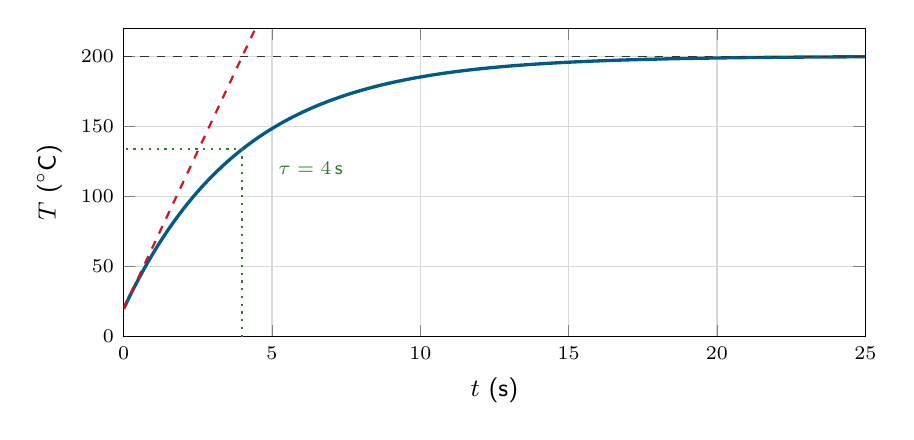
\begin{tikzpicture}
\begin{axis}[width=11cm, height=5.5cm, xmin=0, xmax=25, ymin=0, ymax=220, grid=major, major grid style={gray!30},
  xlabel={$t$ (s)}, ylabel={$T$ ($^\circ$C)}, tick label style={font=\scriptsize}, label style={font=\small}]
\addplot[uimmblue, very thick, domain=0:25, samples=150] {200-180*exp(-x/4)};
\addplot[uimmred, thick, dashed, domain=0:4.6] {20+45*x};
\addplot[uimmgray, dashed] coordinates {(0,200)(25,200)};
\addplot[uimmgreen, dotted, thick] coordinates {(4,0)(4,133.8)(0,133.8)};
\node[font=\scriptsize, uimmgreen] at (axis cs:6.3,120) {$\tau = 4$\,s};
\end{axis}
\end{tikzpicture}
\end{center}

\cor{5}{Seconds membres non constants}
\begin{enumerate}
\item
\begin{enumerate}
\item $\theta_p' = \beta$ : $\beta + 0{,}2\,(\beta t + \gamma) = 2t$. Identification : $0{,}2\,\beta = 2$ donc $\beta = 10$ ; $\beta + 0{,}2\,\gamma = 0$ donc $\gamma = -50$. \res{\theta_p(t) = 10\,t - 50}.
\item $\theta = C\,e^{-0{,}2t} + 10\,t - 50$, $\theta(0) = 20 \Rightarrow C = 70$ : \res{\theta(t) = 70\,e^{-0{,}2t} + 10\,t - 50}.
\item Pour $t$ grand, $\theta(t) \approx 10\,t - 50 = 10\,(t - 5)$ : la pièce suit la rampe avec \res{5\ \text{min}} de retard, ce qui est exactement $\tau = \frac{1}{0{,}2}$. C'est l'erreur de traînage d'un système du premier ordre soumis à une rampe.
\end{enumerate}
\item
\begin{enumerate}
\item $-\lambda e^{-t} + 2\lambda e^{-t} = 3e^{-t}$ donc $\lambda = 3$. Puis $y = C\,e^{-2t} + 3\,e^{-t}$ et $y(0) = 0 \Rightarrow C = -3$ :
\[ \res{y(t) = 3\,e^{-t} - 3\,e^{-2t}} \]
\item $y'(t) = -3e^{-t} + 6e^{-2t} = 3e^{-2t}\,(2 - e^{t})$. Positive pour $t < \ln 2$, négative après. Maximum en \res{t = \ln 2 \approx 0{,}69\ \text{h}} (environ $42$\,min), valeur $y(\ln 2) = \frac32 - \frac34 = \res{0{,}75\ \text{mol/L}}$.
\end{enumerate}
\end{enumerate}

% ============================================================
\partie{Partie B : applications physiques et industrielles}
% ============================================================

\cor{6}{Chute d'un composant avec frottement de l'air}
\begin{enumerate}
\item Sur l'axe orienté vers le bas : $P = +m\,g$ et $f = -k\,v$. Newton : $m\,v' = m\,g - k\,v$, donc \res{m\,v' + k\,v = m\,g}.
\item $v' + 0{,}2\,v = 9{,}81$ ; \res{\tau = \frac{m}{k} = 5\ \text{s}}.
\item $v_p = \frac{9{,}81}{0{,}2} = 49{,}05$ ; $v = 49{,}05 + C\,e^{-0{,}2t}$, $C = -49{,}05$ : \res{v(t) = 49{,}05\,\big(1 - e^{-0{,}2t}\big)}.
\item \res{v_{\lim} = \frac{m g}{k} = 49{,}05\ \text{m/s}} soit $49{,}05 \times 3{,}6 \approx 176{,}6$\,km/h.
\item $1 - e^{-0{,}2t} = 0{,}95 \iff t = 5\ln 20 \approx \res{15{,}0\ \text{s}}$. Comme $\ln 20 \approx 3{,}00$, on retrouve $3\tau = 15$\,s.
\item Non : près de $180$\,km/h, le frottement de l'air est essentiellement proportionnel à $v^2$. Le modèle linéaire est acceptable au début de la chute seulement. Transition vers l'exercice 19.
\end{enumerate}
\vig{Le signe de la force de frottement dépend de l'orientation de l'axe. Faire écrire le bilan des forces vectoriel avant de projeter.}

\cor{7}{Temporisation par circuit RC dans une armoire de robot}
\begin{enumerate}
\item $E = R\,i + u_C = R\,C\,u_C' + u_C$.
\item \res{\tau = 10^4 \times 220\times 10^{-6} = 2{,}2\ \text{s}}.
\item $u_C = 24 + C_1 e^{-t/2{,}2}$, $u_C(0) = 0$ : \res{u_C(t) = 24\,\big(1 - e^{-t/2{,}2}\big)}.
\item $e^{-t_1/2{,}2} = \frac{24 - 15}{24} = 0{,}375$, donc $t_1 = 2{,}2\ln\frac83 \approx \res{2{,}16\ \text{s}}$.
\item $i = C\,u_C' = \frac{E}{R}\,e^{-t/\tau}$ : \res{i(t) = 2{,}4\times 10^{-3}\,e^{-t/2{,}2}\ \text{A}} ; $i(0) = 2{,}4$\,mA (le condensateur déchargé se comporte comme un fil).
\item $t_1 = R\,C\ln\frac83$ donne $R = \dfrac{1}{220\times10^{-6}\times\ln(8/3)} \approx 4\,634\ \Omega$. Valeur E12 la plus proche : \res{4{,}7\ \text{k}\Omega}, d'où $t_1 = 4\,700\times 220\times10^{-6}\times\ln\frac83 \approx \res{1{,}01\ \text{s}}$.
\end{enumerate}

\cor{8}{Refroidissement d'un engrenage après traitement thermique}
\begin{enumerate}
\item $T' + a\,T = 20\,a$ : $T_p = 20$ ; $T = 20 + C\,e^{-at}$ ; $T(0) = 820 \Rightarrow C = 800$.
\item $20 + 800\,e^{-10a} = 505 \iff e^{-10a} = \frac{485}{800} \iff a = \frac{1}{10}\ln\frac{800}{485} \approx \res{0{,}050\ \text{min}^{-1}}$.
\item $T(30) = 20 + 800\,e^{-1{,}5} \approx \res{198{,}5\,^\circ\text{C}}$.
\item $800\,e^{-0{,}05t} < 35 \iff t > 20\ln\frac{800}{35} \approx \res{62{,}6\ \text{min}}$.
\item $T = 30 + 790\,e^{-0{,}05t} < 55 \iff t > 20\ln\frac{790}{25} \approx \res{69{,}1\ \text{min}}$, soit $6{,}5$\,min de plus. Plus l'ambiance se rapproche du seuil, plus l'attente s'allonge. Si l'atelier était à $55\,^\circ$C ou plus, le seuil ne serait jamais atteint.
\item \py{} Sortie avec \texttt{dt = 5} (extrait) :
\begin{sortie}
10 min : 470.0 °C   exact : 505.2 °C\\
20 min : 273.1 °C   exact : 314.3 °C\\
30 min : 162.4 °C   exact : 198.5 °C\\
60 min : 45.3 °C   exact : 59.8 °C
\end{sortie}
\begin{enumerate}
\item À $30$\,min : écart d'environ $36\,^\circ$C.
\item Les points d'Euler sont tous \textbf{au-dessous} de la courbe exacte. L'écart est maximal vers $t = 20$\,min (environ $41\,^\circ$C), puis diminue car les deux courbes tendent vers $20\,^\circ$C. La courbe exacte est convexe (décroissante, avec une pente qui s'adoucit) : la tangente utilisée à chaque pas passe sous la courbe, donc Euler sous-estime systématiquement la température.
\item Avec \texttt{dt = 1} : $191{,}7\,^\circ$C contre $198{,}5\,^\circ$C, écart d'environ $7\,^\circ$C (maximum $7{,}5\,^\circ$C vers $22$\,min). Sur le graphique, les points se serrent et collent presque à la courbe. L'erreur diminue à peu près proportionnellement au pas.
\end{enumerate}
\begin{center}
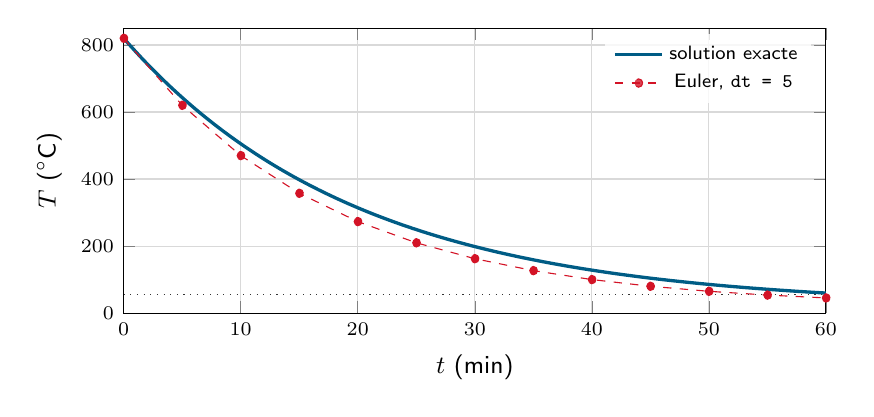
\begin{tikzpicture}
\begin{axis}[width=10.5cm, height=5.2cm, xmin=0, xmax=60, ymin=0, ymax=850, grid=major, major grid style={gray!30},
  xlabel={$t$ (min)}, ylabel={$T$ ($^\circ$C)}, tick label style={font=\scriptsize}, label style={font=\small},
  legend style={font=\scriptsize, draw=none, fill=white, fill opacity=0.8, text opacity=1}]
\addplot[uimmblue, very thick, domain=0:60, samples=120] {20+800*exp(-0.05*x)};
\addlegendentry{solution exacte}
\addplot[uimmred, dashed, mark=*, mark size=1.5pt] coordinates {(0,820)(5,620)(10,470)(15,357.5)(20,273.1)(25,209.8)(30,162.4)(35,126.8)(40,100.1)(45,80.1)(50,65.1)(55,53.8)(60,45.3)};
\addlegendentry{Euler, \texttt{dt = 5}}
\addplot[uimmgray, dotted] coordinates {(0,55)(60,55)};
\end{axis}
\end{tikzpicture}
\end{center}
\item Le rayonnement ajoute une perte de chaleur, forte à haute température. Le refroidissement réel est donc plus rapide au début : le modèle de Newton \textbf{sous-estime} la vitesse de refroidissement initiale.
\end{enumerate}

\cor{9}{Moteur de l'axe J1 d'un robot FANUC}
\begin{enumerate}
\item En divisant par $f$ : $\frac{J}{f}\,\omega' + \omega = \frac{K u}{f}$. \res{\tau = \frac{J}{f} = 2\ \text{s}} ; \res{\Omega_0 = \frac{0{,}5 \times 12}{0{,}01} = 600\ \text{rad/s}}.
\item \res{\omega(t) = 600\,\big(1 - e^{-t/2}\big)}.
\item $\omega'(0) = \frac{\Omega_0}{\tau} = 300\ \text{rad/s}^2$ : la tangente atteint l'asymptote en $t = \tau = 2$\,s.
\end{enumerate}
\begin{center}
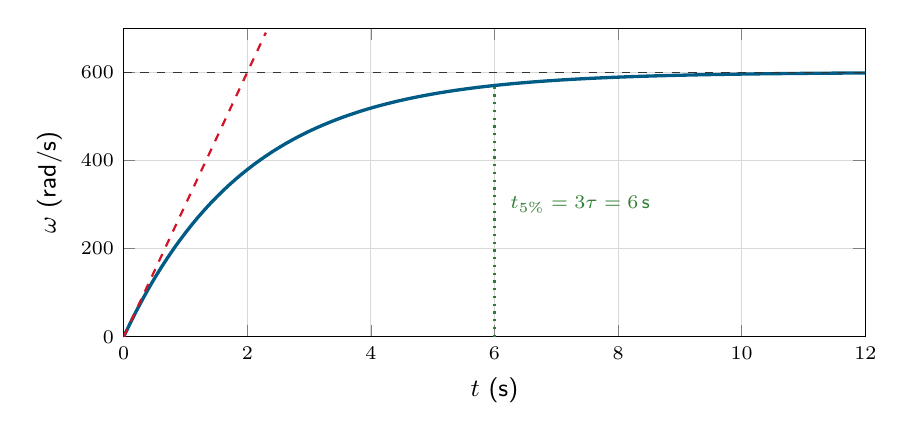
\begin{tikzpicture}
\begin{axis}[width=11cm, height=5.5cm, xmin=0, xmax=12, ymin=0, ymax=700, grid=major, major grid style={gray!30},
  xlabel={$t$ (s)}, ylabel={$\omega$ (rad/s)}, tick label style={font=\scriptsize}, label style={font=\small}]
\addplot[uimmblue, very thick, domain=0:12, samples=120] {600*(1-exp(-x/2))};
\addplot[uimmred, thick, dashed, domain=0:2.3] {300*x};
\addplot[uimmgray, dashed] coordinates {(0,600)(12,600)};
\addplot[uimmgreen, dotted, thick] coordinates {(6,0)(6,570)};
\node[font=\scriptsize, uimmgreen, anchor=west] at (axis cs:6.1,300) {$t_{5\%} = 3\tau = 6$\,s};
\end{axis}
\end{tikzpicture}
\end{center}
\begin{enumerate}[resume]
\item $t_{5\%} = \tau\ln 20 \approx \res{6\ \text{s}}$ ($3\tau$).
\item Non, $6\ \text{s} > 0{,}6\ \text{s}$. Avec $f' = 0{,}1$ et $K' = 5$ : $\tau' = \frac{J}{f'} = 0{,}2$\,s ; $\Omega_0' = \frac{5 \times 12}{0{,}1} = 600$\,rad/s (inchangée). $t_{5\%} = 3\tau' = 0{,}6$\,s (plus précisément $0{,}2\ln 20 \approx 0{,}599$\,s) : le cahier des charges est \textbf{tout juste} respecté, sans marge.
\end{enumerate}
\vig{Modèle simplifié : un vrai moteur à courant continu a aussi une constante de temps électrique, et le couple dépend du courant, pas directement de la tension. Le préciser si un apprenti de spécialité électrotechnique le relève.}

\cor{10}{Ouverture et fermeture d'une électrovanne}
\begin{enumerate}
\item $E = u_R + u_L = R\,i + L\,i'$.
\item \res{\tau = \frac{L}{R} = 0{,}02\ \text{s} = 20\ \text{ms}} ; \res{I_\infty = \frac{E}{R} = 0{,}96\ \text{A}}.
\item \res{i(t) = 0{,}96\,\big(1 - e^{-50t}\big)}. $0{,}96\,(1 - e^{-50t}) = 0{,}6 \iff e^{-50t} = 0{,}375 \iff t = \frac{\ln(8/3)}{50} \approx \res{19{,}6\ \text{ms}}$.
\item $i(t) = 0{,}96\,e^{-50t} < 0{,}2 \iff t > \frac{\ln 4{,}8}{50} \approx \res{31{,}4\ \text{ms}}$.
\item $u_L = L\,i'$ : si le courant passe de $0{,}96$\,A à $0$ en une microseconde, $|u_L| \approx 0{,}5 \times \frac{0{,}96}{10^{-6}} \approx 5\times10^5$\,V. En pratique, cette surtension claque le transistor (ou provoque un arc). La diode de roue libre offre un chemin au courant, qui décroît alors en douceur.
\end{enumerate}

\cor{11}{Filtrer le signal d'un capteur}
\begin{enumerate}
\item $\omega\tau = 1\,000 \times 10^{-3} = 1$. Équation : $10^{-3}\,u' + u = 5\sin(1\,000\,t)$.
\item $u_p' = -1\,000\,\lambda\sin(1\,000t) + 1\,000\,\mu\cos(1\,000t)$, donc $10^{-3}u_p' = -\lambda\sin + \mu\cos$. En reportant :
$(\lambda + \mu)\cos(1\,000t) + (\mu - \lambda)\sin(1\,000t) = 5\sin(1\,000t)$. Identification : $\lambda + \mu = 0$ et $\mu - \lambda = 5$, d'où \res{\lambda = -2{,}5,\ \mu = 2{,}5}.
\item $u = C\,e^{-1\,000t} + u_p$ ; $u(0) = C - 2{,}5 = 0 \Rightarrow C = 2{,}5$ :
\[ \res{u(t) = 2{,}5\,e^{-1\,000t} + 2{,}5\sin(1\,000t) - 2{,}5\cos(1\,000t)} \]
Le transitoire est négligeable après $5\tau = 5$\,ms.
\item $u_p = 2{,}5\sqrt2\,\sin\!\left(1\,000t - \frac{\pi}{4}\right) \approx 3{,}54\sin\!\left(1\,000t - \frac{\pi}{4}\right)$. Amplitude $3{,}54$\,V contre $5$\,V : rapport $\frac{1}{\sqrt2} \approx 0{,}71$, et déphasage de $-\frac{\pi}{4}$. C'est la pulsation de coupure du filtre ($\omega = \frac1\tau$).
\item $\omega\tau = 10$ : $A = \frac{5}{\sqrt{101}} \approx \res{0{,}50\ \text{V}}$. Le parasite est divisé par environ $10$, alors que les signaux lents passent presque intacts : c'est un filtre \textbf{passe-bas}.
\end{enumerate}

% ============================================================
\partie{Partie C : au-delà du cours}
% ============================================================

\cor{12}{Variables séparables : la méthode}
\begin{enumerate}
\item
\begin{enumerate}
\item $x\,\frac{\dd y}{\dd x} = 3y$ ; pour $y \neq 0$ et $x > 0$ : $\frac{\dd y}{y} = 3\,\frac{\dd x}{x}$.
\item $\ln|y| = 3\ln x + \ln|K|$, donc $|y| = |K|\,x^3$ et $y = K\,x^3$ ($K \neq 0$). La fonction nulle vérifie $x \times 0 = 3 \times 0$ : elle correspond à $K = 0$. Solution générale : \res{y = K\,x^3,\ K \in \mathbb{R}}.
\item $y(1) = K = 2$ : \res{y(x) = 2\,x^3}.
\end{enumerate}
\item $y\,\dd y = x\,\dd x$, donc $\frac{y^2}{2} = \frac{x^2}{2} + C$. Avec $y(0) = 2$ : $C = 2$, d'où $y^2 = x^2 + 4$. Comme $y(0) > 0$ et que $y^2 \geq 4$ ne s'annule jamais, $y$ reste positive : \res{y(x) = \sqrt{x^2 + 4}} (branche de l'hyperbole $y^2 - x^2 = 4$).
\item
\begin{enumerate}
\item $\frac{\dd y}{y^2} = 2x\,\dd x$. La dérivée de $-\frac1y$ par rapport à $y$ est $\frac{1}{y^2}$.
\item $-\frac1y = x^2 + C$ ; $y(0) = 1$ donne $C = -1$, donc $\frac1y = 1 - x^2$ : \res{y(x) = \frac{1}{1 - x^2}}.
\item La solution est définie sur $]-1\,;\,1[$ et $y(x) \to +\infty$ quand $x \to 1^-$ : la solution « explose » en un point où l'équation, elle, n'a aucune singularité. Une équation linéaire à coefficients continus a des solutions définies sur tout l'intervalle : ce phénomène est propre au non linéaire.
\end{enumerate}
\end{enumerate}
\vig{En 1b, sans l'astuce $\ln|K|$, beaucoup écrivent $y = x^3 + C$ : la constante additive du logarithme devient multiplicative après passage à l'exponentielle.}

\cor{13}{Usure d'un bain de traitement de surface (cinétique d'ordre 2)}
\begin{enumerate}
\item L'inconnue apparaît au carré. Pour $c \neq 0$ : $\frac{\dd c}{c^2} = -k\,\dd t$, les variables sont séparées.
\item $-\frac1c = -k\,t + C$ ; en $t = 0$ : $C = -\frac{1}{c_0}$. Donc \res{\frac{1}{c(t)} = \frac{1}{c_0} + k\,t} et \res{c(t) = \frac{c_0}{1 + k\,c_0\,t} = \frac{2}{1 + 0{,}1\,t}}.
\item $c = \frac{c_0}{2} \iff k\,c_0\,t = 1 \iff t_{1/2} = \frac{1}{0{,}05 \times 2} = \res{10\ \text{min}}$.
\item $\frac{1}{0{,}1} = \frac12 + 0{,}05\,t \iff t = \frac{9{,}5}{0{,}05} = \res{190\ \text{min}}$.
\item $t_{1/2} = \frac{1}{k c_0}$ ; avec $c_0 = 4$ : $t_{1/2} = 5$\,min (deux fois plus court). Pour l'ordre 1, $t_{1/2}$ ne dépend pas de $c_0$. D'après la question 2, $\frac1c$ est une fonction affine de $t$ : tracer $\frac1c$ en fonction de $t$ donne une droite de pente $k$ pour une cinétique d'ordre 2 (pour l'ordre 1, c'est $\ln c$ qui est affine).
\end{enumerate}

\cor{14}{Vidange d'un réservoir de lubrifiant (loi de Torricelli)}
\begin{enumerate}
\item L'inconnue apparaît sous une racine carrée : l'équation n'est pas linéaire. La forme $y' + \alpha y = f$ n'est pas reconnaissable et la solution n'est pas exponentielle.
\item
\begin{enumerate}
\item $u' = \dfrac{h'}{2\sqrt h} = \dfrac{-k\sqrt h}{2\sqrt h} = -\dfrac k2 = -0{,}05$.
\item $u$ est affine : $u(t) = \sqrt{1{,}5} - 0{,}05\,t$, et $h = u^2$ : \res{h(t) = \big(\sqrt{1{,}5} - 0{,}05\,t\big)^2}.
\end{enumerate}
\item $h'(t) = 2\big(\sqrt{1{,}5} - 0{,}05t\big)\times(-0{,}05) = -0{,}1\big(\sqrt{1{,}5} - 0{,}05t\big)$. Or $\sqrt{h(t)} = \sqrt{1{,}5} - 0{,}05t$ tant que cette quantité est positive. Donc $h' = -k\sqrt h$.
\item $\sqrt{1{,}5} - 0{,}05\,T_v = 0 \iff T_v = 20\sqrt{1{,}5} \approx \res{24{,}5\ \text{min}}$.
\item Mi-hauteur : $\sqrt{0{,}75} \approx 0{,}866$, donc $t = \frac{1{,}2247 - 0{,}8660}{0{,}05} \approx \res{7{,}17\ \text{min}}$.\\
Alarme : $\sqrt{0{,}1} \approx 0{,}316$, donc $t = \frac{1{,}2247 - 0{,}3162}{0{,}05} \approx \res{18{,}17\ \text{min}}$.
\item \py{} Sortie :
\begin{sortie}
Alarme déclenchée à t = 18.17 min
\end{sortie}
Accord avec le calcul exact.
\item Le modèle linéaire donne une décroissance exponentielle : le réservoir ne se vide jamais, et la durée de demi-vidange est toujours la même. Avec Torricelli, la vidange ralentit quand la pression baisse, mais elle se termine en un temps fini. Pour un écoulement par gravité, Torricelli est le modèle physique. Le modèle linéaire correspond à une pompe dont le débit est asservi au niveau.
\end{enumerate}
\begin{center}
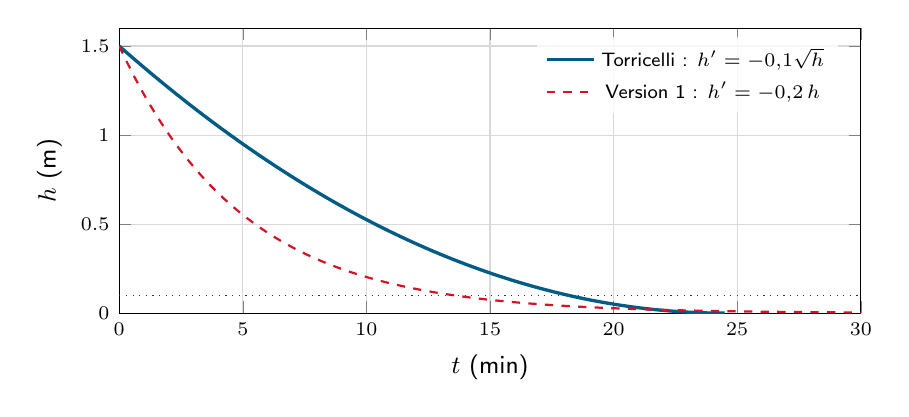
\begin{tikzpicture}
\begin{axis}[width=11cm, height=5.2cm, xmin=0, xmax=30, ymin=0, ymax=1.6, grid=major, major grid style={gray!30},
  xlabel={$t$ (min)}, ylabel={$h$ (m)}, tick label style={font=\scriptsize}, label style={font=\small},
  legend style={font=\scriptsize, draw=none, fill=white, fill opacity=0.8, text opacity=1}, legend pos=north east]
\addplot[uimmblue, very thick, domain=0:24.49, samples=100] {(sqrt(1.5)-0.05*x)^2};
\addlegendentry{Torricelli : $h' = -0{,}1\sqrt h$}
\addplot[uimmred, thick, dashed, domain=0:30, samples=100] {1.5*exp(-0.2*x)};
\addlegendentry{Version 1 : $h' = -0{,}2\,h$}
\addplot[uimmgray, dotted] coordinates {(0,0.1)(30,0.1)};
\end{axis}
\end{tikzpicture}
\end{center}

\cor{15}{Dépollution d'une cuve à volume variable}
\begin{enumerate}
\item $V'(t) = -5$ donc \res{V(t) = 1\,000 - 5\,t}. La cuve est vide pour $t = 200$\,min.
\item $m' = -\frac{25\,m}{1\,000 - 5t} = -\frac{5\,m}{200 - t}$, d'où $m' + \frac{5}{200 - t}\,m = 0$. Le coefficient de $m$ dépend de $t$ : la formule $C\,e^{-\alpha t}$ ne s'applique pas.
\item
\begin{enumerate}
\item Dérivée d'une composée : $\big(\ln m\big)' = \frac{m'}{m}$. En divisant l'équation par $m > 0$ : $\frac{m'}{m} = -\frac{5}{200 - t}$.
\item $\big(5\ln(200 - t)\big)' = 5 \times \frac{-1}{200 - t} = -\frac{5}{200 - t}$.
\item $\ln m$ et $5\ln(200 - t)$ ont la même dérivée sur $[0\,;\,200[$ : elles diffèrent d'une constante $c$. Donc $m = e^{c}\,e^{5\ln(200-t)} = A\,(200 - t)^5$ avec $A = e^c > 0$.
\item $m(0) = A \times 200^5 = 5$, d'où $A = \frac{5}{200^5}$ et \res{m(t) = 5\left(\frac{200 - t}{200}\right)^5}.
\end{enumerate}
\item En grammes, $m = 5\,000\left(\frac{200 - t}{200}\right)^5$ et $V = 5\,(200 - t)$. Donc $c = \frac{5\,000\,(200 - t)^5}{200^5 \times 5\,(200 - t)} = \frac{1\,000}{200}\left(\frac{200 - t}{200}\right)^4 = 5\left(\frac{200 - t}{200}\right)^4$ g/L. Contrôle : $c(0) = 5$\,g/L $= \frac{5\ \text{kg}}{1\,000\ \text{L}}$.
\item $\left(\frac{200 - t}{200}\right)^4 = 0{,}1 \iff \frac{200 - t}{200} = 0{,}1^{1/4} \approx 0{,}5623$, donc \res{t_s = 200\,(1 - 0{,}1^{1/4}) \approx 87{,}5\ \text{min}}. Volume restant : $1\,000 - 5 \times 87{,}5 \approx \res{562\ \text{L}}$.
\item \py{} Sortie :
\begin{sortie}
c < 0,5 g/L après 87.5 min ; volume restant : 562 L
\end{sortie}
\item $m = 5\,e^{-0{,}02t}$ et $c = 5\,e^{-0{,}02t}$ g/L. $c = 0{,}5 \iff t = 50\ln 10 \approx \res{115{,}1\ \text{min}}$, avec $1\,000$\,L à traiter ensuite. Le réglage $Q_s = 25$\,L/min atteint le seuil plus tôt ($87{,}5$\,min) et laisse moins de volume dans la cuve ($562$\,L). Les volumes pompés vers le traitement sont voisins : $25 \times 87{,}5 \approx 2\,190$\,L contre $20 \times 115{,}1 \approx 2\,300$\,L.
\item $m(t) \to 0$ quand $t \to 200$ : quand la cuve est vide, il ne reste plus de solvant. C'est cohérent avec l'hypothèse d'un mélange homogène. En pratique, des dépôts sur les parois échappent au modèle.
\end{enumerate}
\vig{À la question 3c, l'argument « même dérivée sur un intervalle, donc différence constante » doit être explicité : c'est le cœur de la méthode de séparation des variables.}

\cor{16}{Une équation homogène : $y' = (y/x)^2$}
\begin{enumerate}
\item Pour $x > 0$ : $y' = \frac{y^2}{x^2} = \left(\frac yx\right)^2$. Non linéaire (terme $y^2$). $y'$ s'exprime comme fonction de $\frac yx$ seul : équation homogène.
\item
\begin{enumerate}
\item $y = t\,x$ donc $y' = t'\,x + t$.
\item $t + x\,t' = t^2$, d'où \res{x\,t' = t^2 - t}. Variables séparables : $\frac{t'}{t^2 - t} = \frac1x$.
\end{enumerate}
\item
\begin{enumerate}
\item $t = 0$ donne $y = 0$ ($0 = 0$) ; $t = 1$ donne $y = x$ ($x^2 \times 1 = x^2$). Ce sont des solutions particulières (droites).
\item $\frac{1}{t-1} - \frac1t = \frac{t - (t - 1)}{t(t-1)} = \frac{1}{t^2 - t}$.
\item $\ln|t - 1| - \ln|t| = \ln x + \ln|K|$, donc $\left|\frac{t-1}{t}\right| = |K|\,x$ et $\frac{t-1}{t} = K\,x$.
\item $1 - \frac1t = Kx$ donc $t = \frac{1}{1 - Kx}$ et \res{y = \frac{x}{1 - Kx}} (sur un intervalle où $1 - Kx \neq 0$). $K = 0$ redonne $y = x$.
\end{enumerate}
\item $y(1) = \frac{1}{1 - K} = \frac12 \Rightarrow K = -1$ : \res{y(x) = \frac{x}{1 + x}}. $y' = \frac{(1 + x) - x}{(1 + x)^2} = \frac{1}{(1 + x)^2}$ et $x^2 y' = \frac{x^2}{(1 + x)^2} = y^2$.
\item Pour $K < 0$ : $y = \frac{1}{\frac1x - K} \to -\frac1K$ quand $x \to +\infty$ ($0{,}5$ pour $K = -2$, $1$ pour $K = -1$, $2$ pour $K = -0{,}5$). Pour $K = 0$, $y = x$ n'a pas de limite finie.
\item $-\frac1y = -\frac1x + C$, donc $\frac1y = \frac{1 - Cx}{x}$ et $y = \frac{x}{1 - Cx}$ : même famille avec $C = K$. La séparation directe marche ici parce que $f(t) = t^2$ donne $y' = y^2 \times \frac{1}{x^2}$, un produit. Pour $y' = f\!\left(\frac yx\right)$ quelconque (par exemple $y' = \frac yx + \left(\frac yx\right)^2$), les variables ne se séparent pas directement et le changement $y = t\,x$ devient nécessaire (cet exemple est d'ailleurs aussi une équation de Bernoulli).
\end{enumerate}
\vig{Cette équation est à la fois homogène et à variables séparables. La question 6 le fait constater ; l'exemple $y' = \frac yx + \left(\frac yx\right)^2$ peut servir de prolongement : $x\,t' = t^2$, puis $y = \frac{x}{C - \ln x}$.}

\cor{17}{Contamination d'un fluide de coupe (modèle logistique)}
\begin{enumerate}
\item $N' \approx 0{,}8\,N$ : $N \approx 10^3\,e^{0{,}8t}$. $10^3 e^{0{,}8t} = 10^6 \iff t = \frac{\ln 1\,000}{0{,}8} \approx \res{8{,}63\ \text{jours}}$.
\item Pour $N = 0$ et $N = K$, $N' = 0$ et le second membre est nul. $K$ est la concentration maximale que le fluide peut atteindre (saturation) : c'est le régime permanent.
\item
\begin{enumerate}
\item C'est le changement de Bernoulli $z = N^{1-\alpha}$ avec $\alpha = 2$. $z' = -\frac{N'}{N^2}$ (dérivée de $\frac1u$). Puis $z' = -\frac{r N (1 - N/K)}{N^2} = -\frac{r}{N} + \frac{r}{K} = -r\,z + \frac rK$, soit \res{z' + r\,z = \frac rK}.
\item $z = \frac1K + C\,e^{-rt}$ ; $z(0) = 10^{-3}$ donne $C = 10^{-3} - 10^{-8}$. \res{z(t) = 10^{-8} + \big(10^{-3} - 10^{-8}\big)e^{-0{,}8t}}.
\item $N = \dfrac1z = \dfrac{1}{\frac1K + \left(\frac1{N_0} - \frac1K\right)e^{-rt}}$. En multipliant numérateur et dénominateur par $K$ :
\[ \res{N(t) = \frac{K}{1 + \left(\frac{K}{N_0} - 1\right)e^{-rt}}} \]
\end{enumerate}
\item $1 + 99\,999\,e^{-0{,}8t} = 100 \iff t = \frac{1}{0{,}8}\ln\frac{99\,999}{99} \approx \res{8{,}65\ \text{jours}}$. Très proche de $8{,}63$ : jusqu'au seuil, $\frac NK \leq 1\,\%$, donc l'approximation $1 - \frac NK \approx 1$ est excellente.
\item $\left(\frac{K}{N_0} - 1\right)e^{-rt} = 1 \iff t = \frac{\ln 99\,999}{0{,}8} \approx \res{14{,}4\ \text{jours}}$.
\item \py{} Sortie du premier programme :
\begin{sortie}
Seuil de 1 000 000 UFC/mL atteint après 8.69 jours
\end{sortie}
\begin{enumerate}
\item $8{,}69$ contre $8{,}65$ jours : écart dû au pas d'Euler (avec \texttt{dt = 0.001}, on obtient $8{,}65$).
\item Toutes les courbes ont la même forme en S et la même limite $K$. Elles sont décalées dans le temps : multiplier $N_0$ par $10$ avance la courbe de $\frac{\ln 10}{0{,}8} \approx 2{,}9$ jours. Une émulsion neuve dans un circuit mal nettoyé démarre avec un $N_0$ élevé et atteint le seuil plusieurs jours plus tôt. Nettoyer le circuit fait gagner ces jours.
\end{enumerate}
\end{enumerate}
\begin{center}
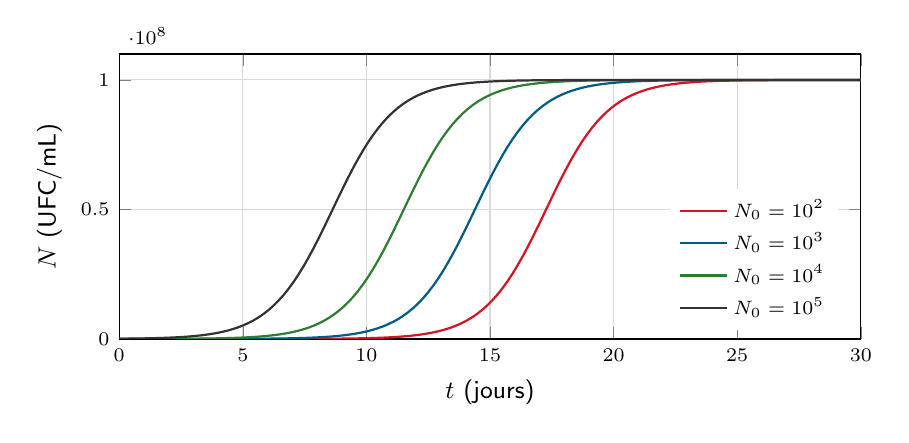
\begin{tikzpicture}
\begin{axis}[width=11cm, height=5.2cm, xmin=0, xmax=30, ymin=0, ymax=1.1e8, grid=major, major grid style={gray!30},
  xlabel={$t$ (jours)}, ylabel={$N$ (UFC/mL)}, tick label style={font=\scriptsize}, label style={font=\small},
  legend style={font=\scriptsize, draw=none}, legend pos=south east]
\foreach \n/\c in {100/uimmred, 1000/uimmblue, 10000/uimmgreen, 100000/uimmgray}{
  \edef\tmp{\noexpand\addplot[\c, thick, domain=0:30, samples=150] {1e8/(1+(1e8/\n-1)*exp(-0.8*x))};}\tmp
}
\legend{$N_0 = 10^2$, $N_0 = 10^3$, $N_0 = 10^4$, $N_0 = 10^5$}
\end{axis}
\end{tikzpicture}
\end{center}
\vig{Les valeurs de $r$, $K$ et du seuil sont choisies pour l'exercice. Elles donnent des ordres de grandeur plausibles mais ne constituent pas une norme de surveillance des fluides de coupe.}

\cor{18}{Ralentissement d'un volant d'inertie (équation de Bernoulli)}
\begin{enumerate}
\item En divisant par $J$ : $\omega' = -0{,}1\,\omega - 0{,}002\,\omega^2$, soit $\omega' + 0{,}1\,\omega = -0{,}002\,\omega^2$. \res{a = 0{,}1,\ b = -0{,}002,\ \alpha = 2}.
\item
\begin{enumerate}
\item $z = \omega^{-1}$ donc $z' = -\omega^{-2}\,\omega' = -\frac{\omega'}{\omega^2}$.
\item $\frac{\omega'}{\omega^2} + \frac{0{,}1}{\omega} = -0{,}002$, soit $-z' + 0{,}1\,z = -0{,}002$ : \res{z' - 0{,}1\,z = 0{,}002}.
\end{enumerate}
\item $z_h = C\,e^{0{,}1t}$, $z_p = -0{,}02$. $z(0) = C - 0{,}02 = \frac{1}{300}$ donne $C = \frac{7}{300}$.\\
$z = \frac{7e^{0{,}1t} - 6}{300}$, d'où \res{\omega(t) = \frac{300}{7\,e^{0{,}1t} - 6}}. Contrôle : $\omega(0) = 300$.
\item $7\,e^{0{,}1t} - 6 = 10 \iff t = 10\ln\frac{16}{7} \approx \res{8{,}3\ \text{s}}$.
\item $300\,e^{-0{,}1t} = 30 \iff t = 10\ln 10 \approx \res{23{,}0\ \text{s}}$. À $300$\,rad/s : $f\omega = 15$\,N$\cdot$m et $c\,\omega^2 = 90$\,N$\cdot$m. Le couple aérodynamique est six fois plus fort à haute vitesse : le ralentissement initial est bien plus rapide.
\item Pour $t$ grand, $7\,e^{0{,}1t} \gg 6$, donc $\omega \approx \frac{300}{7}\,e^{-0{,}1t}$ : décroissance exponentielle, comme le modèle linéaire. À basse vitesse, $\frac{c\,\omega^2}{f\,\omega} = 0{,}02\,\omega < 1$ dès que $\omega < 50$\,rad/s : le frottement visqueux domine.
\end{enumerate}
\vig{Signe de $b$ : il est négatif. Une erreur de signe donne $z' + 0{,}1 z = \dots$ et une solution qui ne vérifie plus $\omega(0) = 300$ de façon cohérente : faire contrôler $\omega(0)$.}

\cor{19}{Essai de chute d'un boîtier : frottement quadratique}
\begin{enumerate}
\item $m\,v' = m\,g - k\,v^2$, d'où $v' = g - \frac{k}{m}v^2$. Le terme $v^2$ rend l'équation non linéaire.
\item $v' \approx g = 9{,}81\ \text{m/s}^2$ : au début, c'est une chute libre, $v \approx g\,t$.
\item $g - \frac km v_{\lim}^2 = 0$ donne $v_{\lim} = \sqrt{\frac{m g}{k}} = \sqrt{981} \approx \res{31{,}3\ \text{m/s}}$, soit environ $113$\,km/h.
\item \py{} Sortie :
\begin{sortie}
v\_lim = 31.32 m/s\\
95 \% de v\_lim à t = 5.85 s ; chute de 116.4 m
\end{sortie}
\item $v'(t) = v_{\lim}\times\frac{g}{v_{\lim}}\left(1 - \tanh^2\frac{g t}{v_{\lim}}\right) = g\left(1 - \frac{v^2}{v_{\lim}^2}\right) = g - \frac{g}{v_{\lim}^2}\,v^2$. Or $\frac{g}{v_{\lim}^2} = \frac{g\,k}{m\,g} = \frac km$ : on retrouve $v' = g - \frac km v^2$. Et $v(0) = v_{\lim}\tanh 0 = 0$.
\item $\frac{g\,t}{v_{\lim}} = 1{,}832 \iff t = \frac{1{,}832 \times 31{,}32}{9{,}81} \approx \res{5{,}85\ \text{s}}$, comme la simulation.
\end{enumerate}
\vig{La notion de constante de temps $\tau$ du cours n'existe plus ici : la règle « $95\,\%$ à $3\tau$ » ne s'applique pas à une équation non linéaire.}

\cor{20}{Problème : refroidissement avec rayonnement}
\begin{enumerate}
\item $820\,^\circ\text{C} = 1\,093$\,K ; $20\,^\circ\text{C} = 293$\,K ; $55\,^\circ\text{C} = 328$\,K. La loi de Stefan porte sur la température absolue : en degrés Celsius, $T^4 - T_e^4$ changerait de valeur (un décalage d'origine ne conserve pas les puissances quatrièmes).
\item À $t = 0$ : convection $-0{,}03 \times 800 = -24$\,K/min ; rayonnement $-1{,}4\times10^{-10}\times(1\,093^4 - 293^4) \approx -199$\,K/min. À $100\,^\circ$C ($373$\,K) : $-2{,}4$\,K/min contre $-1{,}7$\,K/min. Le rayonnement domine nettement au début (environ huit fois plus), la convection à la fin.
\item L'équation est autonome : $\dfrac{\dd T}{-a(T - T_e) - b(T^4 - T_e^4)} = \dd t$. Il faudrait une primitive de l'inverse d'un polynôme de degré 4 (factorisation et décomposition en éléments simples très lourdes), et l'on obtiendrait $t$ en fonction de $T$ sans pouvoir isoler $T$. Euler s'impose.
\item \py{} Sortie :
\begin{sortie}
Pièce à 55 °C après 46.1 min
\end{sortie}
Newton seul avec $a = 0{,}03$ : $t = \frac{1}{0{,}03}\ln\frac{800}{35} \approx 104$\,min. Exercice 8 ($a = 0{,}05$ calé sur une mesure) : $62{,}6$\,min. Le rayonnement divise la durée par plus de deux par rapport à la seule convection. Le modèle calé de l'exercice 8 se situe entre les deux : il compense en moyenne le rayonnement, sans en reproduire la forme. Repère : à $10$\,min, le modèle complet donne environ $264\,^\circ$C (calcul avec un pas fin), contre $613\,^\circ$C pour Newton seul.
\item Avec \texttt{dt = 5}, le programme affiche « 5 min ». Premier pas : $T_1 = 1\,093 + 5 \times (-24 - 199) \approx -21$\,K, en dessous du zéro absolu : résultat absurde. Le pas est trop grand devant la rapidité de l'évolution initiale : en linéarisant, $\left|\frac{\partial}{\partial T}\right| \approx a + 4bT^3 \approx 0{,}76\ \text{min}^{-1}$ à $1\,093$\,K, et le schéma d'Euler n'est stable que pour $\Delta t < \frac{2}{0{,}76} \approx 2{,}6$\,min. Règle pratique : diviser le pas par deux jusqu'à ce que le résultat ne change plus ($44$\,min avec \texttt{dt = 1}, $46{,}1$\,min avec \texttt{dt = 0.01}).
\end{enumerate}
\vig{Le critère de stabilité $\Delta t < \frac{2}{\lambda}$ n'est pas au programme : il peut être donné oralement aux plus avancés. L'essentiel est la démarche « réduire le pas et comparer ».}

\end{document}
